
%\title{Modelo de Projeto de pesquisa}
%% abtex2-modelo-projeto-pesquisa.tex, v-1.9 laurocesar
%% Copyright 2012-2013 by abnTeX2 group at http://abntex2.googlecode.com/ 
%%
%% This work may be distributed and/or modified under the
%% conditions of taTeX Project Public License, either version 1.3
%% of this license or (at your option) any later version.
%% The latest version of this license is in
%%   http://www.latex-project.org/lppl.txt
%% and version 1.3 or later is part of all distributions of LaTeX
%% version 2005/12/01 or later.
%%
%% This work has the LPPL maintenance status `maintained'.
%% 
%% The Current Maintainer of this work is the abnTeX2 team, led
%% by Lauro César Araujo. Further information are available on 
%% http://abntex2.googlecode.com/
%%
%% This work consists of the files abntex2-modelo-projeto-pesquisa.tex
%% and abntex2-modelo-references.bib
%%

% ------------------------------------------------------------------------
% ------------------------------------------------------------------------
% abnTeX2: Modelo de Projeto de pesquisa em conformidade com 
% ABNT NBR 15287:2011 Informação e documentação - Projeto de pesquisa -
% Apresentação 
% ------------------------------------------------------------------------ 
% ------------------------------------------------------------------------

\documentclass[
	% -- opções da classe memoir --
	12pt,				% tamanho da fonte
	openany,			%openright capítulos começam em pág ímpar (insere página vazia caso preciso)
	oneside,			%twoside para impressão em verso e anverso. Oposto a oneside
	a4paper,			% tamanho do papel. 
	% -- opções da classe abntex2 --
	%chapter=TITLE,		% títulos de capítulos convertidos em letras maiúsculas
	%section=TITLE,		% títulos de seções convertidos em letras maiúsculas
	%subsection=TITLE,	% títulos de subseções convertidos em letras maiúsculas
	%subsubsection=TITLE,% títulos de subsubseções convertidos em letras maiúsculas
	% -- opções do pacote babel --
	english,			% idioma adicional para hifenização
	french,				% idioma adicional para hifenização
	spanish,			% idioma adicional para hifenização
	brazil,				% o último idioma é o principal do documento
	]{abntex2}

% ---
% PACOTES
% ---

% ---
% Pacotes fundamentais 
% ---
\usepackage{lmodern}			% Usa a fonte Latin Modern
\usepackage[T1]{fontenc}		% Selecao de codigos de fonte.
\usepackage[utf8]{inputenc}		% Codificacao do documento (conversão automática dos acentos)
\usepackage{indentfirst}		% Indenta o primeiro parágrafo de cada seção.
\usepackage{color}				% Controle das cores
\usepackage{graphicx}			% Inclusão de gráficos
\usepackage{microtype} 			% para melhorias de justificação
\usepackage{tikz}
\usepackage{float}
\usetikzlibrary{shapes,arrows}
% ---

% ---
% Pacotes adicionais, usados apenas no âmbito do Modelo Canônico do abnteX2
% ---
\usepackage{lipsum}				% para geração de dummy text
% ---

% ---
% Pacotes de citações
% ---
\usepackage[brazilian,hyperpageref]{backref}	 % Paginas com as citações na bibl
\usepackage[alf]{abntex2cite}	% Citações padrão ABNT

% --- 
% CONFIGURAÇÕES DE PACOTES
% --- 

% ---
% Configurações do pacote backref
% Usado sem a opção hyperpageref de backref
\renewcommand{\backrefpagesname}{Citado na(s) página(s):~}
% Texto padrão antes do número das páginas
\renewcommand{\backref}{}
% Define os textos da citação
\renewcommand*{\backrefalt}[4]{
	\ifcase #1 %
		Nenhuma citação no texto.%
	\or
		Citado na página #2.%
	\else
		Citado #1 vezes nas páginas #2.%
	\fi}%
% ---

% ---
% Informações de dados para CAPA e FOLHA DE ROSTO
% ---
\titulo{Um estudo de caso do uso de mineração de dados e aprendizado de máquina
  no aprimoramento de  inspeções de estações radio base} \autor{Marcelo Veloso
  Maciel} \local{Brasil}

\instituicao{%
  Universidade de Pernambuco -- UPE
  \par
  Residência Tecnológica em Inteligência Artificial}
\tipotrabalho{Trabalho de conclusão}
% O preambulo deve conter o tipo do trabalho, o objetivo, 
% o nome da instituição e a área de concentração 
\preambulo{Trabalho de conclusão}
% ---

% ---
% Configurações de aparência do PDF final

% alterando o aspecto da cor azul
\definecolor{blue}{RGB}{41,5,195}

% informações do PDF
\makeatletter
\hypersetup{
     	%pagebackref=true,
		pdftitle={\@title}, 
		pdfauthor={\@author},
    	pdfsubject={\imprimirpreambulo},
	    pdfcreator={LaTeX with abnTeX2},
		pdfkeywords={abnt}{latex}{abntex}{abntex2}{projeto de pesquisa}, 
		colorlinks=true,       		% false: boxed links; true: colored links
    	linkcolor=blue,          	% color of internal links
    	citecolor=blue,        		% color of links to bibliography
    	filecolor=magenta,      		% color of file links
		urlcolor=blue,
		bookmarksdepth=4
}
\makeatother
% --- 

% --- 
% Espaçamentos entre linhas e parágrafos 
% --- 

% O tamanho do parágrafo é dado por:
\setlength{\parindent}{1.3cm}

% Controle do espaçamento entre um parágrafo e outro:
\setlength{\parskip}{0.2cm}  % tente também \onelineskip

% ---
% compila o indice
% ---
\makeindex
% ---

% ----
% Início do documento
% ----
\begin{document}

% Retira espaço extra obsoleto entre as frases.
\frenchspacing 

% ----------------------------------------------------------
% ELEMENTOS PRÉ-TEXTUAIS
% ----------------------------------------------------------
% \pretextual

% ---
% Capa
% ---
\imprimircapa
% ---

% ---
% Folha de rosto
% ---
\imprimirfolhaderosto
% ---

% ---
% NOTA DA ABNT NBR 15287:2011, p. 4:
%  ``Se exigido pela entidade, apresentar os dados curriculares do autor em
%     folha ou página distinta após a folha de rosto.''
% ---

% ---
% inserir lista de ilustrações
% ---
\pdfbookmark[0]{\listfigurename}{lof}
\listoffigures*
\cleardoublepage
% ---

% ---
% inserir lista de tabelas
% ---
\pdfbookmark[0]{\listtablename}{lot}
\listoftables*
\cleardoublepage
% ---

% ---
% inserir lista de abreviaturas e siglas
% ---
% ---

% ---
% inserir o sumario
% ---
\pdfbookmark[0]{\contentsname}{toc}
\tableofcontents*
\cleardoublepage
% ---


% ----------------------------------------------------------
% ELEMENTOS TEXTUAIS
% ----------------------------------------------------------
\textual

% ----------------------------------------------------------
% Introdução
% ----------------------------------------------------------
\chapter*[Introdução]{Introdução}
\addcontentsline{toc}{chapter}{Introdução}

%\backrefsetup{disable}

Nas últimas décadas a temática do impacto social da inteligência artificial vem
tomando centralidade no imaginário prospectivo do cidadão médio, da comunidade
científica e dos agentes estatais \cite{cameron1991terminator,
  cockburn2018impact, makridakis2017forthcoming}. A ascensão do assunto na
opinião pública não é desconexa de mudanças no contexto econômico e político
\cite{kogut2003global}. A difusão da internet na sociedade, culminando nas
tecnologias IoT \cite{gubbi2013internet}, faz com que dados passem a ser
consideradas pela The Economist \footnote{Fonte:
  \url{https://tinyurl.com/y39u52kk}.
  Acessado em 1 de Novembro de 2019 .} o novo petróleo.

Esse papel dos dados pressupõe a capacidade dos agentes econômicos de extrair
valor deles. É essa a seara de inserção dos algoritmos de inteligência
computacional, particularmente os de aprendizado de máquina. Algoritmos de
aprendizado de máquina são aqueles que aprendem com uma experiência com relação
a alguma tarefa e uma medida de performance se a performance na tarefa melhora
com a experiência \cite{carbonell1984machine}. Se os dados são o novo petróleo
então os algoritmos utilizados para extrair informação e aprender com esses
dados podem ser considerados os novos motores da economia.


O presente estudo apresenta um caso de sucesso da aplicação de sistemas
inteligentes de recuperação e análise de informação de relativa simplicidade no
aprimoramento de um processo rotineiro na indústria de telecomunicações: a
inspeção de estações rádio base. \textcolor{red}{O restante do trabalho está
  estruturado da seguinte forma}

\chapter[Descrição do Caso]{Descrição do Caso}
Como referenciado anteriormente o sistema alvo de interesse do nosso estudo está
inserido no âmbito da indústria de telecomunicações. Na rede de celulares a
mediação entre o celular dos usuários e as companhias telefônicas é feita pelas
Estações Rádio Base (doravante ERB ou sítio celular). São nesses sítios que
estão instalados os equipamentos necessários para a comunicação entre aparelhos
celulares e as centrais de comunicação das agências telefônicas. Nesses
ambientes são realizadas vistorias frequentes tendo em vista sua relevância para
a qualidade do serviço de telefonia. Nessas vistorias são checados itens
referentes às chaves do sítio, à rua de acesso, alarmes externos, aterramento,
baterias, cabos, fontes de energia, antenas, dentre centenas outros. Essa
vistoria é um trabalho conjunto entre técnicos que visitam os sítios e
engenheiros de telecomunicação que analisam as informações. Atualmente essa
troca de informação é feita da seguinte maneira: o técnico visita a ERB e para
cada item de um \textit{checklist}, que tem até 600 itens a depender da
empresa de telefonia detentora do sítio, tiram fotos que são enviadas a um
sistema, onde são aceitas ou rejeitadas pelos engenheiros na central. Contudo,
nem todo item precisa ser checado a depender de condições particulares da ERB.
Estes itens são, portanto, abonados.

Em conversas com técnicos e engenheiros responsáveis pelas inspeções foram
identificadas ao menos duas possibilidades de aplicação de inteligência
computacional no aperfeiçoamento do processo: a definição de quais itens são
abonados e quais são aprovadas ou rejeitadas. O problema da dispensa do item,
enfoque do presente trabalho, é que os técnicos não sabem de antemão quais itens
devem ser abonados em um determinado sítio. Ao chegarem a ERB, desta forma,
primeiro devem checar dentre centenas de itens em uma lista quais são
dispensáveis e só então iniciam o trabalho da vistoria propriamente dita. Isso
contribui drasticamente para a lentidão da atividade. Nossa contribuição para a
redução do tempo despendido nessa checagem é descrita em seguida.

\chapter[Solução proposta]{Solução proposta}
Temos por problema a determinação de quais itens de um checklist são passíveis
de abono. Isso pode ser modelado como um problema de classificação binária :
dado um conjunto de características de um sítio e qual o item desejamos prever
se ele é da classe ``abonado'' ou não \cite{james2013introduction}.
Especialistas apontaram a seguinte lista de características de um sítio que os
próprios técnicos usam para abonar manualmente os itens:

\begin{itemize}
\item Tipo de site: 'RT', 'GF', 'RF', 'IN'; 
\item Tipo de tecnologia: WCDMA, LTE, GSM;
\item Frequência: 450Mhz, 700Mhz, 850Mhz, 1800Mhz,  2100Mhz, 2600Mhz;
\item Equipamentos de radiofrequência (RF): Diplex, Triplex, Quadriplex, EHCU, Filtro, TMA, DTMA
\end{itemize}

Essas informações, contudo, não estão prontamente disponíveis. Uma fonte
possível de informação são os Projetos Preliminares de Instalação (PPIs). Eles
estão disponíveis em um sistema interno das empresas de telefonia, ao qual nos
foi dado acesso, em formato pdf. Tivemos acesso também à base de checklists dos
sítios. Identificamos 602 ERBs cadastrada nesse sistema das quais baixamos cerca
de 150 PPIs e os checklists de fevereiro a setembro. Dentre os PPIs foram
identificados 3 padrões de documento. Como um esforço inicial trabalhamos na
extração de informação de um único padrão. Dado esse recorte de um único tipo de
documento, a intersecção entre o grupo de sítios que tínhamos tanto o checklist
quanto o PPI tem uma cardinalidade de 44.

As características das ERBs estavam de presentes de forma não estruturada em
tabelas e textos nos ppis. A informação não contida nas tabelas, extraídas por
meio de pacotes especializados, foi obtida por meio da tokenização dos textos.
Desta forma geramos automaticamente uma base de características dos sítios. A
partir da intersecção entre a base de características e a base de items geramos
um banco de dados de 19000 observações. Na base temos 322 items únicos, com uma
mediana de 243 items por ERB, e 19 atributos ('Items', 'Status', 'Operadora',
'Tipo de Site', 'WCDMA', 'LTE', 'GSM', '450Mhz', '700Mhz', '850Mhz', '1800Mhz',
'2100Mhz', '2600Mhz', 'Diplex', 'Triplex', 'Quadriplexer', 'EHCU', 'Filtro',
'TMA', 'DTMA'), onde todos menos ``Item'' e ``Tipo de Site'' são variáveis
binárias.

Uma inspeção inicial na base nos permitiu identificar um desbalanceamento no
número de itens avaliados x os abonados, no ``Status'' do item. O
desbalanceamento das classes impacta na performance preditiva de modelos, na
medida em que o modelo ganha um viés para a classe majoritária simplesmente pelo
maior número de observações dessa classe, aumentando, portanto, o número de
falso negativos \cite{faceli2011inteligencia}. Como demonstrado na Figura
\ref{ref:figbal} o número de itens abonados era mais do dobro dos itens
avaliados, de forma que optamos pela sobreamostragem da classe minoritária por
meio de um método de interpolação padrão: o SMOTE (Synthetic Minority
Over-sampling Technique) \cite{chawla2002smote}. 

\begin{figure}[h]
  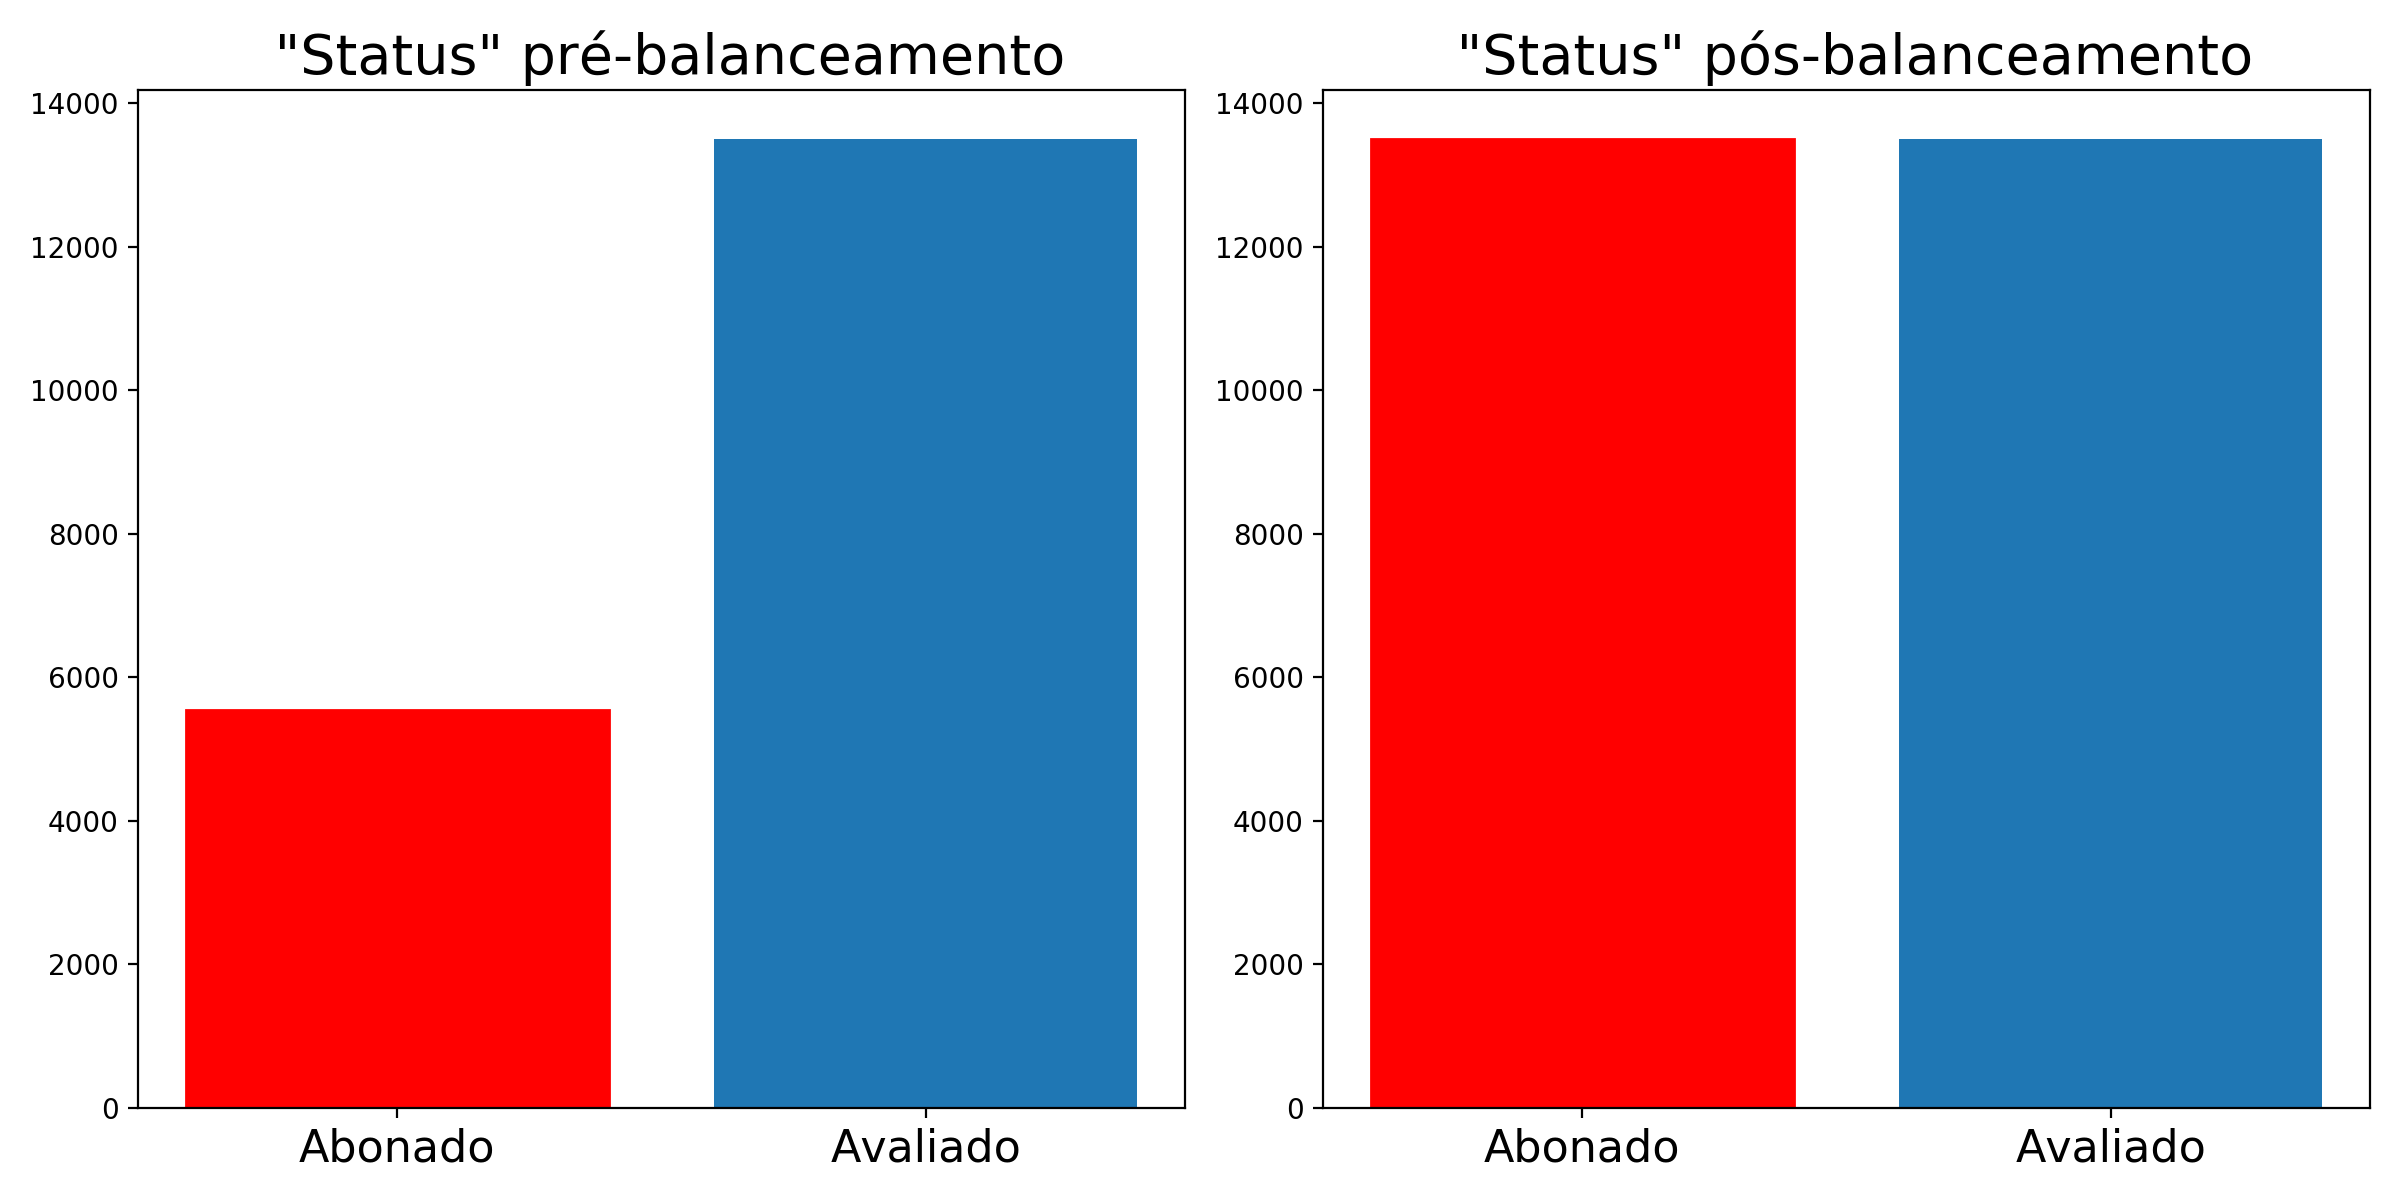
\includegraphics[scale=0.5]{img/balanceamento.png}
  \caption{Número de Abonados vis-à-vis Avaliados pré e pós balanceamento}
  \label{ref:figbal}
\end{figure}

Após o rebalanceamento codificamos os atributos ``Item'' e ``Tipo de Site'' por
meio de one-hot-encoding. Uma outra opção de codificação seria atribuir um
número inteiro a cada item, mas essa estratégia confundiria o modelo ao
implicitamente atribuir ordem a uma variável nominal
\cite{faceli2011inteligencia}.


\begin{figure}[H]
  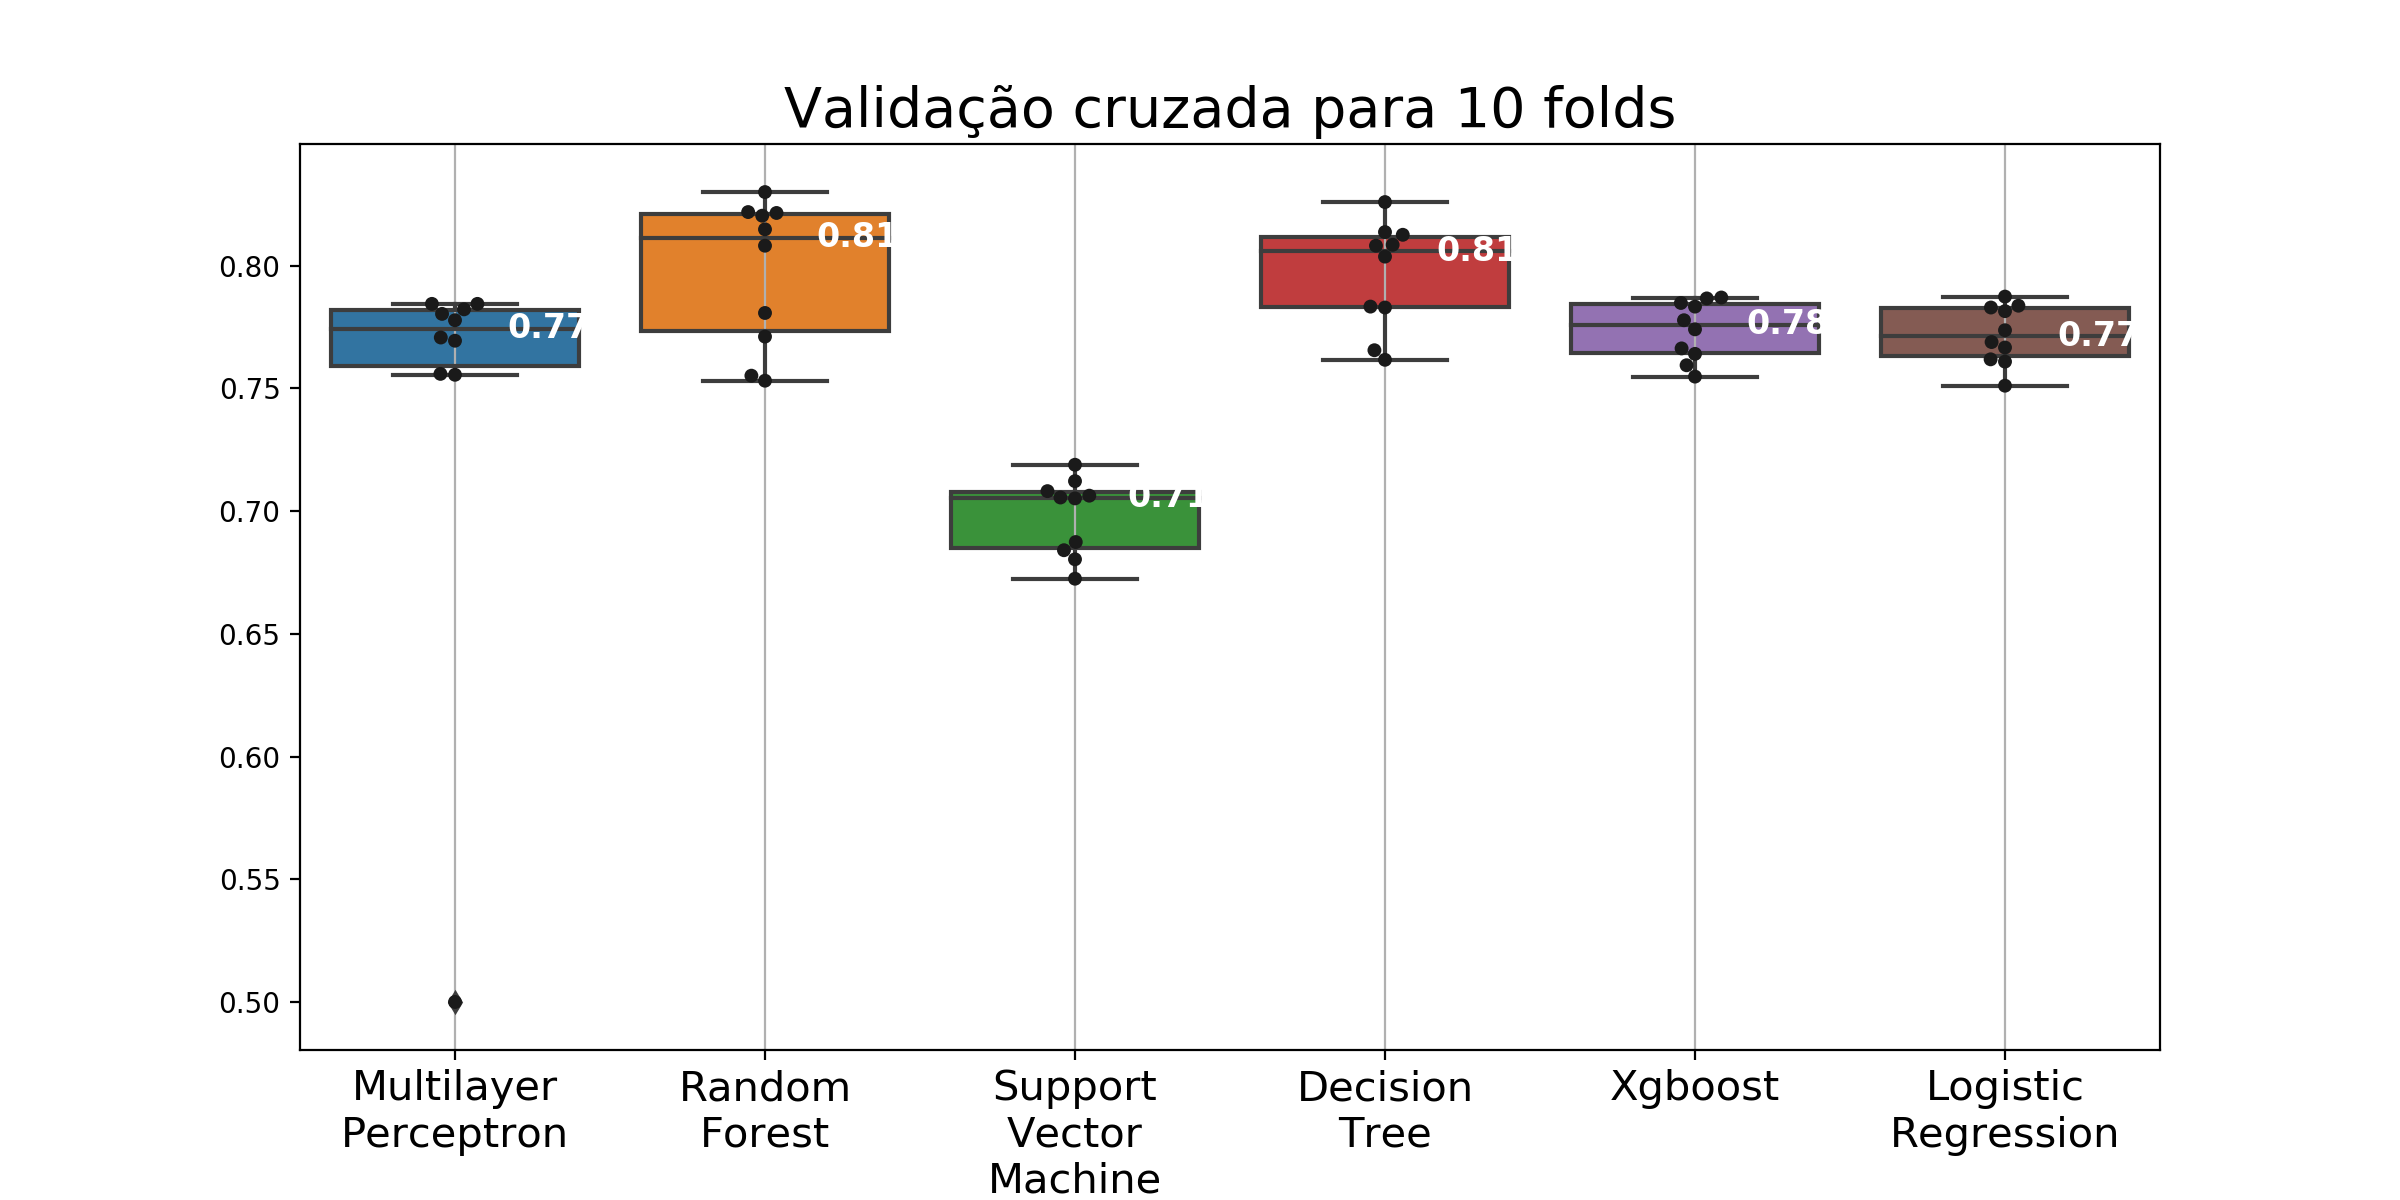
\includegraphics[scale=0.5]{img/cvs.png}
  \caption{Distribuição de acurácias. Acurácia mediana anotada em cada caixa.}
  \label{ref:figaccs}
\end{figure}

Uma vez concluído o preprocessamento partimos para o uso de modelos preditivos
de aprendizado de máquina. Fizemos um Grid Search\footnote{Modelos de
  aprendizado de máquina apresentam parâmetros, conhecidos como hiperparâmetros,
  que não são aprendidos internamente, eles são configura\c{c}ões do modelo. É
  considerada uma boa prática testar diferentes combinações de hiperparâmetros
  para identificar qual parametrização tem a melhor métrica de avaliação. O Grid
  Search é quando testamos exaustivamente as parametrizações estabelecidas
  \cite{geron2019hands}. }, com validação cruzada (k-fold com 10 folds), dos
seguintes modelos: Decision Tree, Multilayer Perceptron, Logistic Regression,
Random Forest, Xgboost. A Figura \ref{ref:figaccs} demonstra a distribuição de
acurácias, (número de predições corretas) / (número total de predições ) , dos
melhores classificadores de cada tipo. A árvore de decisão (Decision Tree) e a
floresta aleatória foram os classificadores com melhor performance. Nossa
hipótese para a performance da Decision Tree é que como o banco de dados após o
preprocessamento só possui variáveis binárias a árvore de decisão, que funciona
por meio de uma árvore de divisões do banco em perguntas binárias, é um
algoritmo ``naturalmente'' eficiente. A floresta aleatória é simplesmente um
conjunto de árvores de decisão. No nosso caso a floresta aleatória tem a mesma
acurácia das árvores de decisão, mas com um custo computacional muito maior. A
árvore de decisão figura então como o algoritmo utilizado em nossa solu\c{c}ão.

A nossa solu\c{c}ão busca auxiliar a tomada de decisão. Desta forma, o output de
interesse dos usuários seria quais itens teriam a maior probabilidade de serem
abonados em determinado sítio. A árvore de decisão nos permite determinar a
probabilidade, para o classificador, de uma instância possuir a uma classe, no
nosso caso a classe ``Status''. Sendo assim nossa solu\c{c}ão é a seguinte:
\begin{enumerate}
\item o usuário indica qual a ERB de inspe\c{c}ão;
\item procuramos na base qual as características do sítio;
\item as características preprocessadas são enviadas ao classificador treinado,
  a árvore de decisão, que retorna as probabilidades de pertencimento à classe
  ``Abonado'' de cada item do site;
  \item retornamos ao usuário a lista ordenada, pela probabilidade decrescente
    de pertencimento à classe, dos itens do site.
\end{enumerate}




\chapter*[Conclusão]{Conclusão}
\addcontentsline{toc}{chapter}{Conclusão}

No presente trabalho apresentamos um caso de aperfei\c{c}oamento do processo de
inspe\c{c}ão de esta{c}ões rádio base por meio de minera\c{c}ão de dados e
inteligência artificial. Embora grandes empresas de tecnologia como Google,
Facebook e Amazon façam uso de grandes arquiteturas de redes neurais artificiais
as quais necessitam de dezenas de horas de treinamento em unidades de
processamento gráfico, a realidade da maior parte das empresas que buscam se
inserir nessa nova era algorítmica difere em escopo \cite{canziani2016analysis}.
Se por um lado a inteligência artificial traz a possibilidade de uma riqueza de
aplicações e otimizações no processo produtivo das empresas, por outro lado se
faz necessária uma infraestrutura de dados que permita a aplicação dessas
técnicas e uma ``pipeline'' de mineração e recuperação de informação
\cite{schutze2007introduction}. Ademais a restrição orçamentária e computacional
e o imperativo da interpretabilidade\footnote{No contexto de aprendizado de
  máquina a interpretabilidade é definida por \citeonline[p.2]{doshi2017towards}
  "como a habilidade de explicar ou apresentar em termos compreensíveis para
  humanos". Uma definição equivalente de interpretabilidade é: o grau no qual um
  humano pode compreender a causa de uma decisão \cite{miller2018explanation}.}
do funcionamento dos algoritmos nos direciona, nesses casos medianos, à
algoritmos mais bem estabelecidos e simples em comparação aos de alta
publicização \cite{dreiseitl2002logistic}.

No nosso caso a minera\c{c}ão de dados contidos em documentos contidos nos
servidores internos de empresas de tecnologias em conjun\c{c}ão com um modelo
simples e interpretável de aprendizado de máquina nos permitiu contribuir no
processo produtivo. Há, contudo, muito a ser feito. Primeiramente, estender a
minera\c{c}ão para todos os tipos de documentos contidos nos servidores é o
próximo passo. Segundo, investigar como melhorar a acurácia dos classificadores,
dado que temos um limiar máximo de aproximadamente 82\%. Nossa hipótese, por
meio de investiga\c{c}ão dos servidores e conversas com usuários, é que o não
cumprimento dos procedimentos de inspe\c{c}ão nas respostas aos itens gera ruído
que confunde os classificadores. A despeito disso, ainda há a necessidade de
investigar como aperfei\c{c}oar os algoritmos independentemente da qualidade dos
dados. Por fim, a determina\c{c} de quais itens são abonáveis é somente a
primeira tarefa, pois o problema de determinar, algoritmicamente, quais itens
são aceitos ou rejeitados há de requerer uma pletora de estudos adicionais.






% ---
% Conclusão
% ---

% ELEMENTOS PÓS-TEXTUAIS
% ----------------------------------------------------------
\postextual

% ----------------------------------------------------------
% Referências bibliográficas
% ----------------------------------------------------------
\bibliography{abntex2-modelo-references}

% ----------------------------------------------------------
% Glossário
% ----------------------------------------------------------
%
% Consulte o manual da classe abntex2 para orientações sobre o glossário.
%
%\glossary
%---------------------------------------------------------------------
% INDICE REMISSIVO
%---------------------------------------------------------------------

\phantompart

\printindex


\end{document}
